\documentclass[aspectratio=169,12pt]{beamer}
\geometry{paperwidth=256mm,paperheight=144mm}
\usepackage{fontspec}
\setsansfont{Latin Modern Sans}
\usefonttheme{professionalfonts}
\usepackage{unicode-math}
\setmathfont{latinmodern-math.otf}
\usepackage[spanish,es-tabla]{babel}
\usepackage{amsmath,booktabs,graphicx}
\definecolor{navy}{HTML}{183650}
\definecolor{accent}{HTML}{B37435}
\definecolor{muted}{HTML}{536477}
\setbeamercolor{normal text}{fg=navy,bg=white}
\setbeamercolor{frametitle}{fg=navy,bg=white}
\setbeamercolor{structure}{fg=accent}
\setbeamertemplate{navigation symbols}{}
\setbeamertemplate{headline}{}
\setbeamersize{text margin left=11mm,text margin right=11mm}
\setbeamerfont{frametitle}{size=\fontsize{27}{32}\selectfont,series=\bfseries}
\setbeamertemplate{frametitle}{\vspace{4mm}\insertframetitle\par\vspace{2mm}\textcolor{accent}{\rule{22mm}{1pt}}}
\newcommand{\maincount}{10}
\newcommand{\backuptotal}{6}
\setbeamertemplate{footline}{\hspace{11mm}{\fontsize{10}{12}\selectfont\color{muted}Beyond Beta\hfill
\ifnum\value{framenumber}>10 Respaldo \number\numexpr\value{framenumber}-10\relax/\backuptotal
\else\insertframenumber/\maincount\fi\hspace{11mm}}\vspace{3mm}}
\newcommand{\slide}[2]{\begin{frame}{#1}\fontsize{22}{27}\selectfont #2\end{frame}}
\newcommand{\captionline}[1]{\par\vspace{1mm}{\fontsize{13}{16}\selectfont\color{muted}#1\par}}
\newcommand{\chart}[2]{\centering\includegraphics[width=\linewidth,height=86mm,keepaspectratio]{figures/#1.pdf}\captionline{#2}}
\newcommand{\backtable}[1]{{\fontsize{17}{21}\selectfont\renewcommand{\arraystretch}{1.35}#1}}
\hypersetup{pdftitle={El CAPM y los modelos multifactoriales en la práctica},pdfauthor={Alonso Castro Freibott, Pablo Caonabo Crespo de la Cruz, Carlos Segovia Domínguez y Jaime Blanco González}}
\begin{document}
\begin{frame}\relax
{\fontsize{17}{21}\selectfont\color{accent}BEYOND BETA}\hfill
\includegraphics[width=73mm]{../../templates/branding/cunef-eps.jpeg}\par\vspace{5mm}
{\fontsize{35}{40}\selectfont\bfseries El CAPM y los modelos\\multifactoriales en la práctica\par}\vspace{5mm}
{\fontsize{23}{28}\selectfont ¿Qué explica el mercado y qué añade FF3?\par}\vspace{7mm}
{\fontsize{17}{22}\selectfont Alonso Castro Freibott · Pablo Caonabo Crespo de la Cruz\par Carlos Segovia Domínguez · Jaime Blanco González\par
Inversiones Financieras\par
Profesor: Javier Fernández Sánchez de la Viña\par}
\end{frame}

\section{Datos}
\slide{Seis activos para comparar exposiciones}{
\begin{columns}[T]
\begin{column}{.55\linewidth}
\backtable{\begin{tabular}{ll}\toprule Activo & Tipo\\\midrule
ACS, Nike, Roblox & Acciones individuales\\
PPFB & ETC de oro físico\\
EUNH & ETF de bonos soberanos\\
IUSQ & ETF de bolsa mundial\\\bottomrule\end{tabular}}
\end{column}
\begin{column}{.41\linewidth}
\textbf{61 precios, 60 retornos}\par\vspace{3mm}
septiembre de 2021 a septiembre de 2026\par\vspace{3mm}
Yahoo Finance y factores de Fama--French\par
\end{column}
\end{columns}\vspace{5mm}
IUSQ forma parte de la cartera. El CAPM se estima con la prima de mercado de EE. UU.
\captionline{IUSQ cotiza en EUR y mantiene la exposición a las divisas de sus inversiones.}
}
\slide{Una muestra común en USD para estimar el CAPM}{
\[\begin{gathered}E(R_i)=R_f+\beta_i[E(R_M)-R_f]\\[2mm]
R_{i,t}-RF_t=\alpha_i+\beta_i(Mkt-RF)_t+\varepsilon_{i,t}\end{gathered}\]
\begin{columns}[T]
\begin{column}{.31\linewidth}
\textbf{Muestra}\par\vspace{2mm}
Último cierre ajustado de cada mercado y mes. Muestra mensual común.
\end{column}
\begin{column}{.31\linewidth}
\textbf{Moneda}\par\vspace{2mm}
Precios en USD. Cambio de la fecha del cierre o de la última fecha disponible anterior.
\end{column}
\begin{column}{.31\linewidth}
\textbf{Estimación}\par\vspace{2mm}
OLS mensual con intercepto y prima de mercado de EE. UU.
\end{column}
\end{columns}
\captionline{octubre de 2021 a septiembre de 2026. RF ya es mensual. Mkt-RF es la prima de mercado, no el retorno total.}
}

\section{Resultados}
\slide{Trayectorias de los activos y la cartera}{
\chart{wealth}{USD, base 100. Cartera: 1/6 por activo, rebalanceo mensual, sin costes ni impuestos. Precios ajustados de Yahoo Finance.}
}
\slide{Rentabilidad y volatilidad anualizadas}{
\chart{risk_return}{La volatilidad resume el riesgo total observado. La beta de la siguiente diapositiva mide sensibilidad al mercado.}
}
\slide{Alfa y beta responden a preguntas distintas}{
\chart{capm_intervals}{Alfa: desviación media mensual. Beta: sensibilidad del exceso del activo a un punto porcentual adicional del factor. Barras: IC del 95\,\% frente a cero.}
}
\slide{La distancia a la SML mide el alfa de Jensen}{
\chart{sml}{Medias aritméticas mensuales USD. Relleno: alfa significativo; cuadrado: beta no significativa. OLS al 5\%.}
}
\slide{Cartera: 7,31 \% anual y -31,88 \% de caída máxima}{
\begin{columns}[T]
\begin{column}{.69\linewidth}
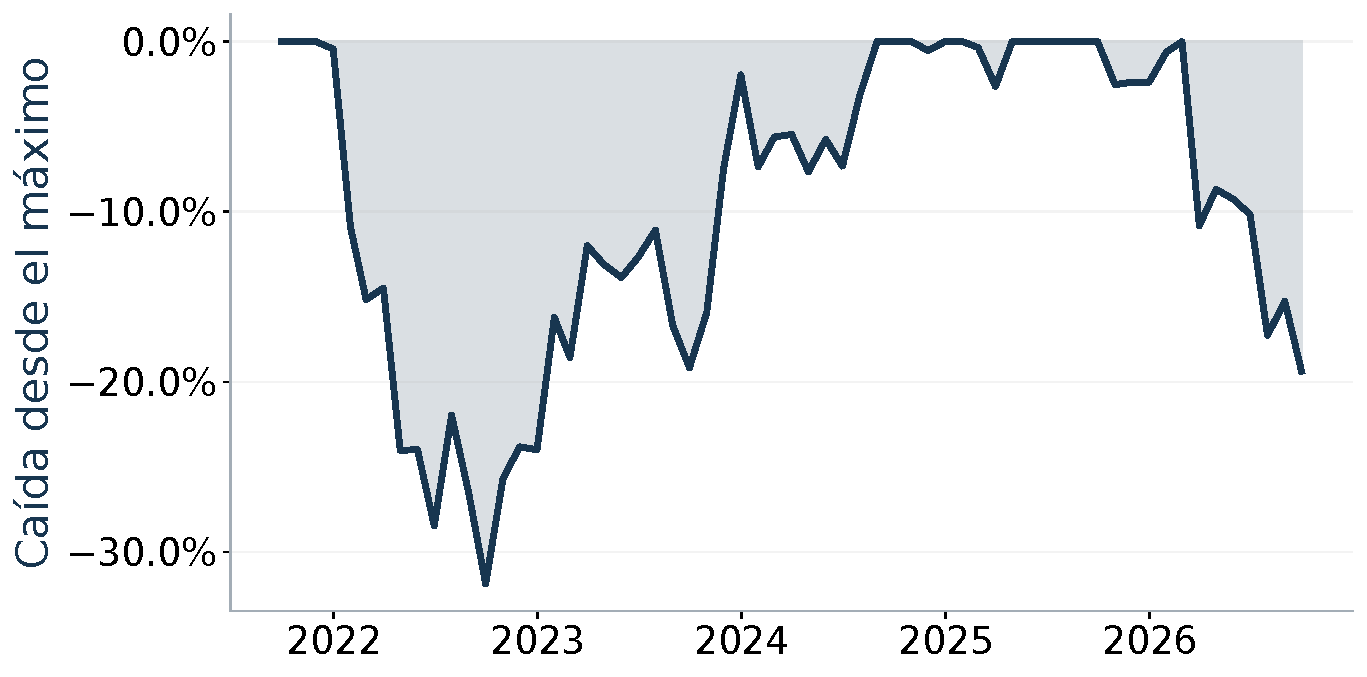
\includegraphics[width=\linewidth,height=80mm,keepaspectratio]{figures/drawdown.pdf}
\end{column}
\begin{column}{.28\linewidth}
\textbf{42,30 \%}\par acumulado\par\vspace{5mm}
\textbf{17,91 \%}\par volatilidad anual\par\vspace{5mm}
\textbf{-31,88 \%}\par caída máxima entre cierres
\end{column}\end{columns}
\captionline{Cartera equiponderada, rebalanceo mensual. Sin costes de negociación ni impuestos. Caída desde el máximo, incluyendo riqueza inicial.}
}
\slide{FF3 no mejora el R\textsuperscript{2} ajustado}{
\begin{columns}[T]
\begin{column}{.61\linewidth}
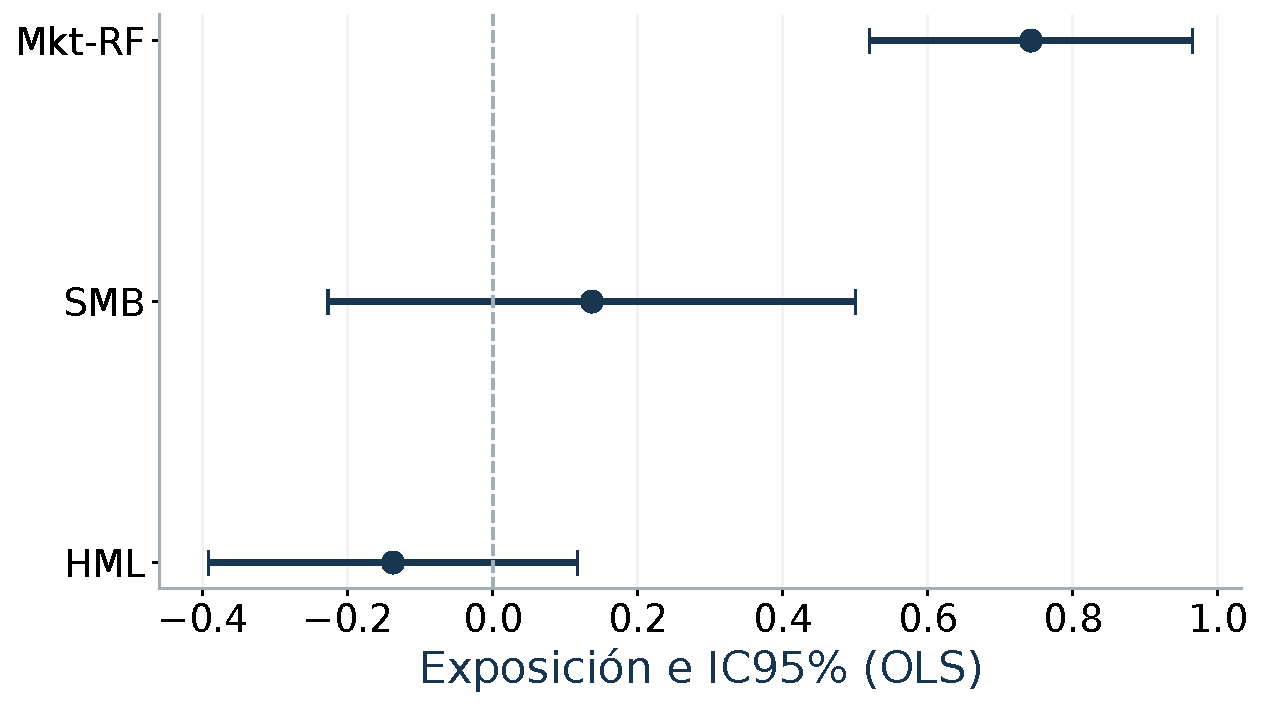
\includegraphics[width=\linewidth,height=80mm,keepaspectratio]{figures/ff3_exposures.pdf}
\end{column}
\begin{column}{.36\linewidth}
\textbf{R\textsuperscript{2} ajustado}\par
CAPM: 0,4882\par FF3: 0,4848\par\vspace{4mm}
\textbf{SMB}\, Pequeñas menos grandes.\par\vspace{2mm}
\textbf{HML}\, Alto menos bajo valor contable/mercado.
\end{column}\end{columns}
\captionline{Beta de mercado: CAPM 0,7888, FF3 0,7425. SMB y HML: evidencia individual insuficiente al 5 \%. Barras: IC del 95\,\%.}
}
\section{Conclusiones}
\slide{En esta cartera, FF3 aporta poco ajuste}{
\begin{enumerate}
\item Alfa significativo: ACS, Nike, Bonos euro. El contraste depende del modelo de referencia.
\item Cartera: 7,31 \% geométrico anual y caída máxima entre cierres mensuales de -31,88 \%.
\item FF3 eleva R\textsuperscript{2}, pero reduce R\textsuperscript{2} ajustado. No encontramos alfa de cartera significativo.
\end{enumerate}\vspace{4mm}
\textcolor{accent}{Límites:} 60 meses, factores de EE. UU. y cierres no simultáneos.
\captionline{Los resultados describen asociaciones históricas.}
}

\appendix
\section{Respaldo}
\slide{A1 · CAPM completo de los seis activos}{
\backtable{\begin{tabular}{lrrrrr}\toprule Activo & $\alpha$ mes (\%) & $p_\alpha$ & $\beta$ & $p_\beta$ & $R^2$\\\midrule
ACS & 2,12 & 0,0176 & 0,696 & 0,0005 & 0,192 \\
Oro PPFB & 1,11 & 0,0896 & 0,165 & 0,2423 & 0,023 \\
Nike & -2,87 & 0,0082 & 1,044 & <0,0001 & 0,267 \\
Roblox & -0,73 & 0,7523 & 1,514 & 0,0034 & 0,139 \\
Bonos euro & -0,89 & 0,0102 & 0,438 & <0,0001 & 0,387 \\
Bolsa mundial & 0,01 & 0,9681 & 0,877 & <0,0001 & 0,921 \\
\bottomrule\end{tabular}}
\captionline{$p_\alpha$: desviación media frente al CAPM. $p_\beta$: sensibilidad a la prima bursátil de EE. UU. $R^2$: proporción de variación explicada. IC del 95\,\% en la diapositiva 6.}
}
\slide{A2 · OLS frente a HAC}{
\backtable{\begin{tabular}{lrrr}\toprule Activo & $p_\alpha$ OLS & $p_\alpha$ HAC & IC95\% HAC de $\alpha$ (\%/mes)\\\midrule
ACS & 0,0176 & 0,0450 & [0,05; 4,19] \\
Oro PPFB & 0,0896 & 0,1164 & [-0,29; 2,51] \\
Nike & 0,0082 & 0,0029 & [-4,72; -1,02] \\
Roblox & 0,7523 & 0,7570 & [-5,40; 3,95] \\
Bonos euro & 0,0102 & 0,0197 & [-1,63; -0,15] \\
Bolsa mundial & 0,9681 & 0,9636 & [-0,27; 0,28] \\
Cartera & 0,6691 & 0,7158 & [-1,34; 0,93] \\
\bottomrule\end{tabular}}
\captionline{Newey--West, Bartlett, 3 retardos, corrección de muestra y distribución t. No cambia qué alfas son significativos al 5 \%.}
}
\slide{A3 · FF3 y CAPM sobre la misma cartera}{
\backtable{\begin{tabular}{lrrrr}\toprule Término & Estimación & $p$ OLS & IC95\% OLS & $p$ HAC\\\midrule
alpha & -0,036 & 0,9437 & [-1,047; 0,975] & 0,9492 \\
Mkt-RF & 0,742 & <0,0001 & [0,519; 0,966] & <0,0001 \\
SMB & 0,137 & 0,4545 & [-0,227; 0,501] & 0,4520 \\
HML & -0,137 & 0,2832 & [-0,392; 0,117] & 0,2503 \\
\bottomrule\end{tabular}}\vspace{3mm}
\backtable{\begin{tabular}{lrrrr}\toprule Modelo & $R^2$ & $R^2$ ajustado & AIC & BIC\\\midrule
CAPM & 0,4969 & 0,4882 & -224,11 & -219,92 \\
FF3 & 0,5110 & 0,4848 & -221,82 & -213,44 \\
\bottomrule\end{tabular}}
\captionline{Alfa en \%/mes. Contraste OLS conjunto de $H_0:\beta_{\mathrm{SMB}}=\beta_{\mathrm{HML}}=0$: $F(2,56)=0,8099$, $p=0,4500$.}
}
\slide{A4 · Rentabilidades, moneda y SML}{
\[P^{USD}_{i,t}=P^{EUR}_{i,t}X_{i,t},\qquad X=\text{USD por EUR}\]
\[R^{USD}_{i,t}=(1+R^{EUR}_{i,t})\frac{X_{i,t}}{X_{i,t-1}}-1\]
\[\overline R_i^{SML}=\overline {RF}+\widehat\beta_i\,\overline {Mkt-RF}\]
\[\overline R_i-\overline R_i^{SML}=\widehat\alpha_i\]
\captionline{4 días de antigüedad FX permitidos, 0 observados. No se divide una rentabilidad por un nivel de cambio. La SML usa medias aritméticas.}
}
\slide{A5 · Diversificación y rebalanceo}{
\(R_{p,t}=\sum_i w_iR_{i,t}\), con 1/6 por activo. \quad \(\widehat\beta_p=\sum_i w_i\widehat\beta_i=0,7888\).
\par\vspace{2mm}\centering
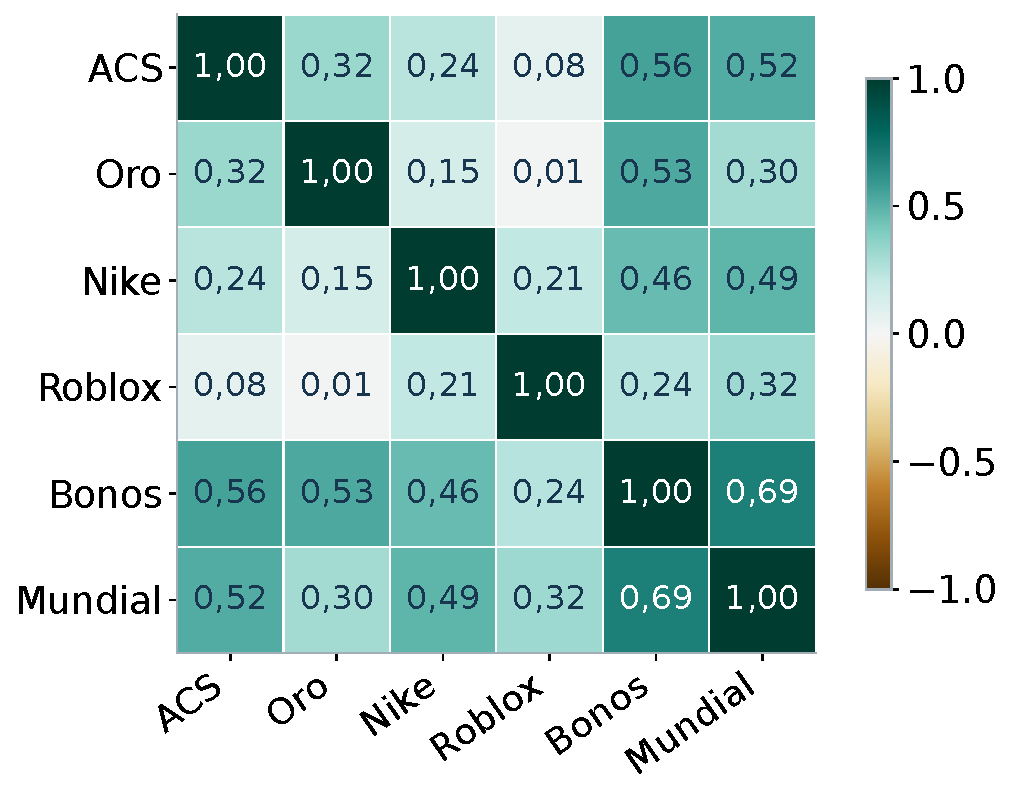
\includegraphics[width=.70\linewidth,height=72mm,keepaspectratio]{figures/correlations.pdf}
\captionline{Beta directa: 0,7888. Mismos meses, moneda, RF y mercado. Los pesos iguales en capital no implican contribuciones iguales al riesgo.}
}
\slide{A6 · Fuentes y límites de interpretación}{
\begin{itemize}
\item Yahoo Finance vía yfinance: cierres ajustados. Fama y French: Copia del profesor, base CRSP 202609.
\item septiembre de 2021 a septiembre de 2026 de precios, octubre de 2021 a septiembre de 2026 de retornos.
\item Tipos, oro y divisas no quedan resumidos por factores bursátiles de EE. UU.
\item 60 meses, contrastes múltiples, precios revisables y calendarios distintos.
\end{itemize}
\captionline{Referencia conceptual: temario de Inversiones Financieras, temas 3 y 4. Factores: \url{https://mba.tuck.dartmouth.edu/pages/faculty/ken.french/data_library/f-f_factors.html}. Fuentes de productos en docs/sources.md.}
}
\end{document}
